%%%%%%%%%%%%%%%%%%%%%%%%
% DO NOT TOUCH THIS PART
\documentclass{hitec}
\newcommand{\HT}{\textsc{\raisebox{0.1em}{h}\raisebox{-0.1em}{i}%
	\raisebox{0.1em}{t}\raisebox{-0.1em}{e}\raisebox{0.1em}{c} }}
	
\usepackage[table,xcdraw]{xcolor}
%%%%%%%%%%%%%%%%%%%%%%%%

\usepackage{tikz}
\usetikzlibrary{arrows}
\usepackage{float}

\usepackage {listings}
% Enter the title of either the lab or some other title you think fits
\title{Application Note Template}

% Place you team members here
\author{Matthew Rainey}




\company{Rowan University}
\confidential{\textbf{-- ECE 09.321: Milestone 2 --}}


% Place the packages you want to use here.
\usepackage{hyperref} % This line is readily ommited of it makes trouble
\usepackage{graphicx}
\tikzstyle{int}=[draw, fill=blue!20, minimum size=2em]
\tikzstyle{init} = [pin edge={to-,thin,black}]


\begin{document}
\maketitle
\section{Design Overview}

This application note demonstrates the operation of a fan controller using a PID controller. This controller has the ability to read from a thermistor and set a fan to a given temperature based off of that read temperature. This temperature is displayed on a 7 segment display. Additionally, the system takes a potentiometer as an input, and displays it on the 7 segment display. This is done while constraining the program to an Attiny13a microcontroller.
\\


\subsection{Design Features}
\begin{itemize}
\item <1 kb program size
\item sleep mode utilization for lowest power consumption possible
\item PID controller to maximize efficiency
\item Thermistor use with an attiny13a for low BOM
\end{itemize}
\subsection{Featured Applications}

A few featured applications of this fan controller are: \\
\begin{itemize}
\item CPU/GPU fans
\item heaters
\item PC case fans
\end{itemize}
\subsection{Design Resources}


This project is open-source and available on request from Matt Rainey. Send an email to Raineym5@students.rowan.edu with the title "PID controller request"

\subsection{Board Image}
Below is a photo of the latest stable design. This includes the microcontroller and surrounding circuitry, thermistor, power regulator, 7 segment display board, USB programmer, resistor, and the fan. The connections for these are all visible.
\begin{figure}[H]
\centering
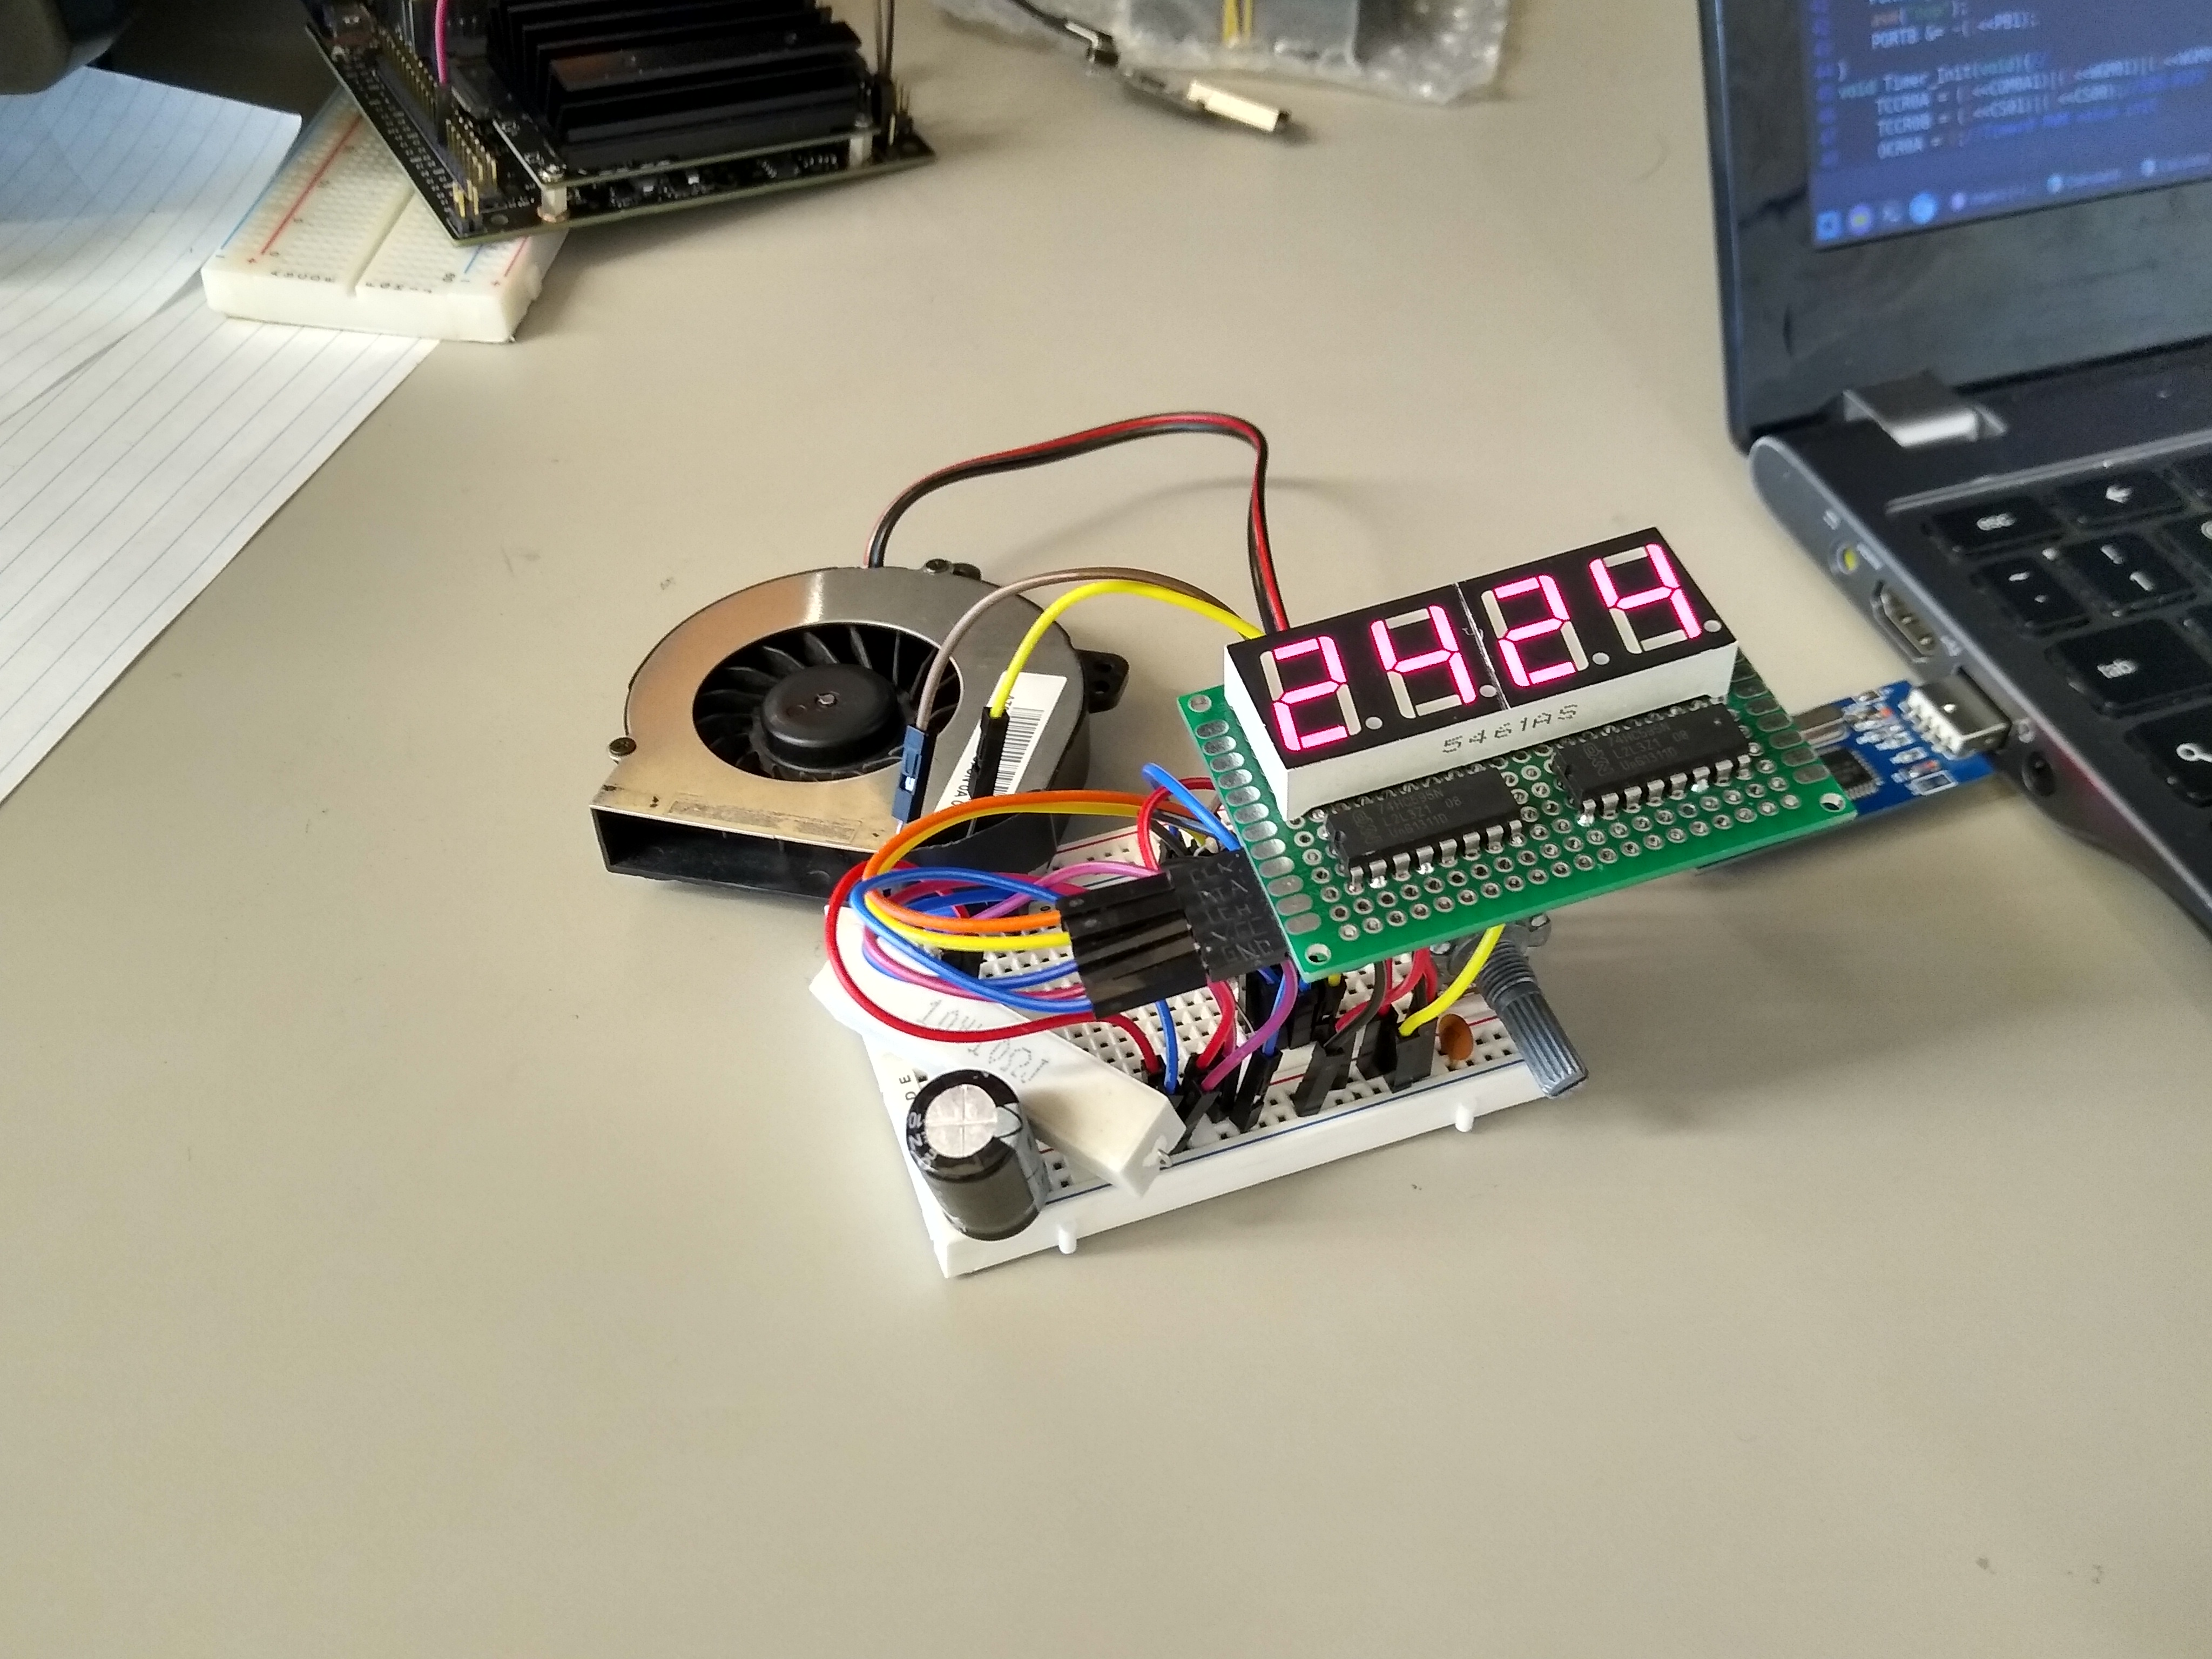
\includegraphics[width=0.9\textwidth]{boardphoto.jpg}
\caption{Photo of latest stable design}
\label{fig:programmerbreadboard}
\end{figure}
Below, a photo of the microcontroller is visible, showing a few of the constraints that were used. 
\begin{figure}[H]
\centering
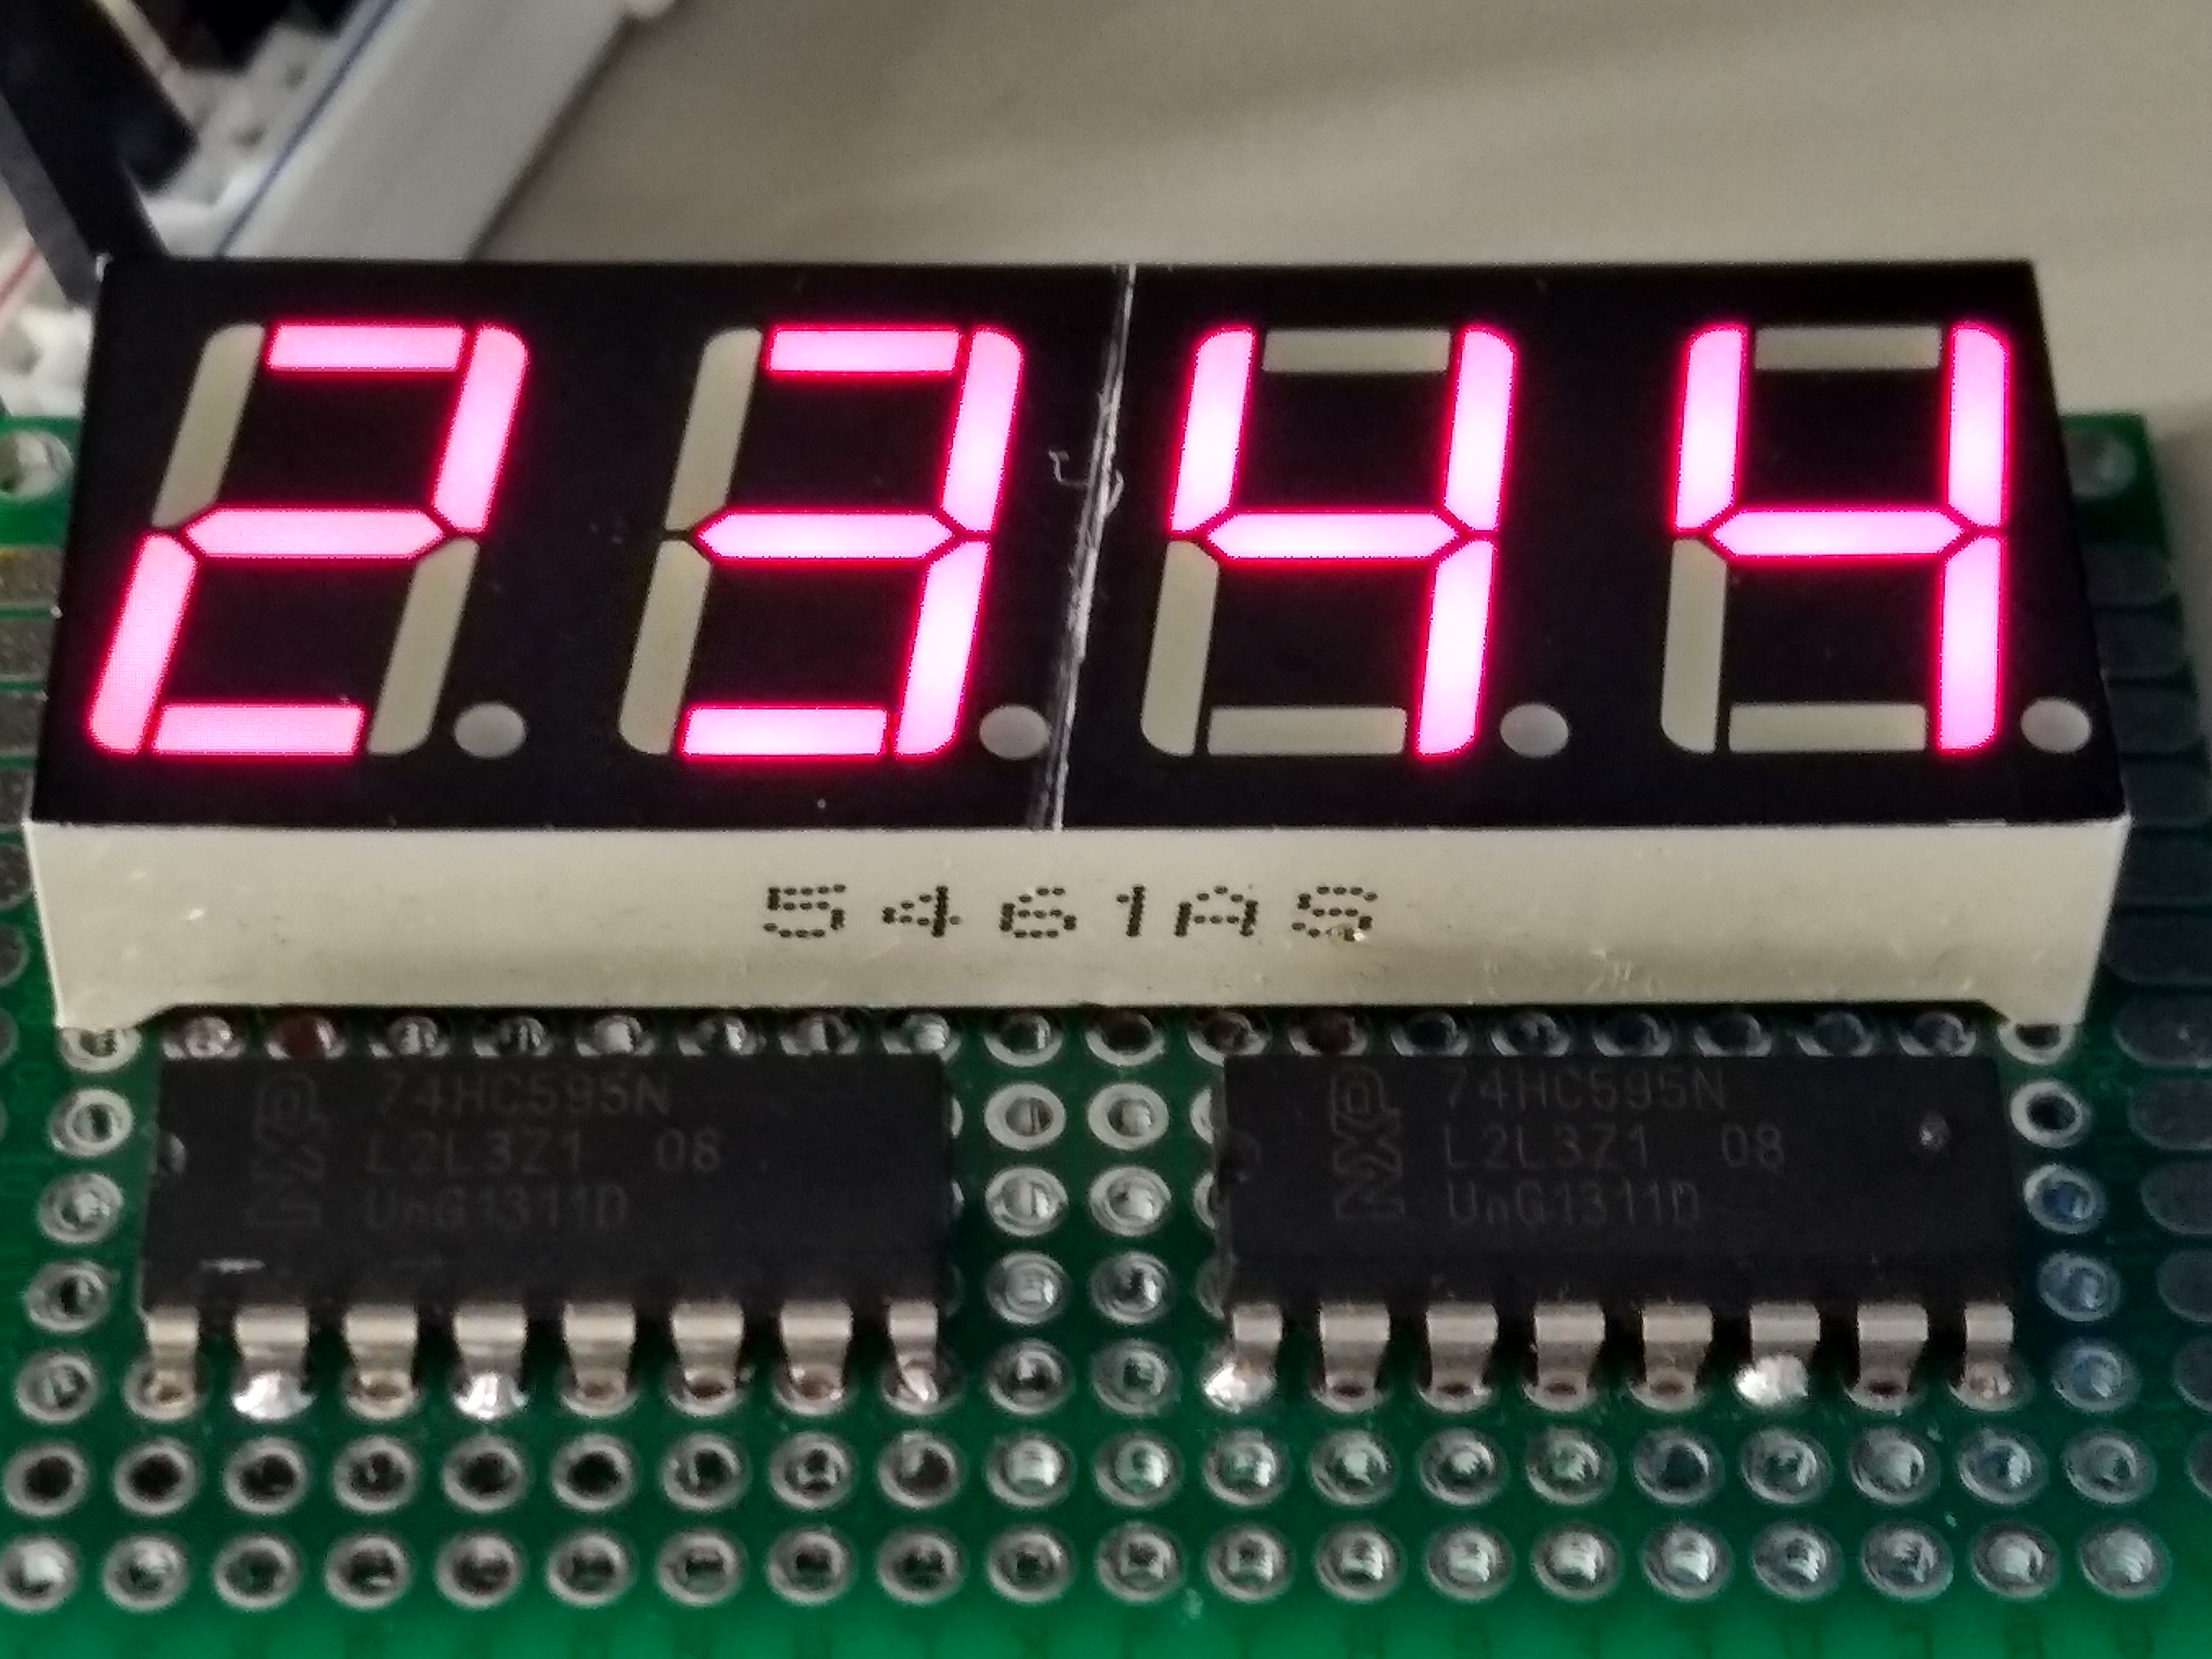
\includegraphics[width=0.9\textwidth]{boardphoto2.jpg}
\caption{7seg board photo}
\label{fig:boardphoto}
\end{figure}
\begin{figure}[H]
\centering
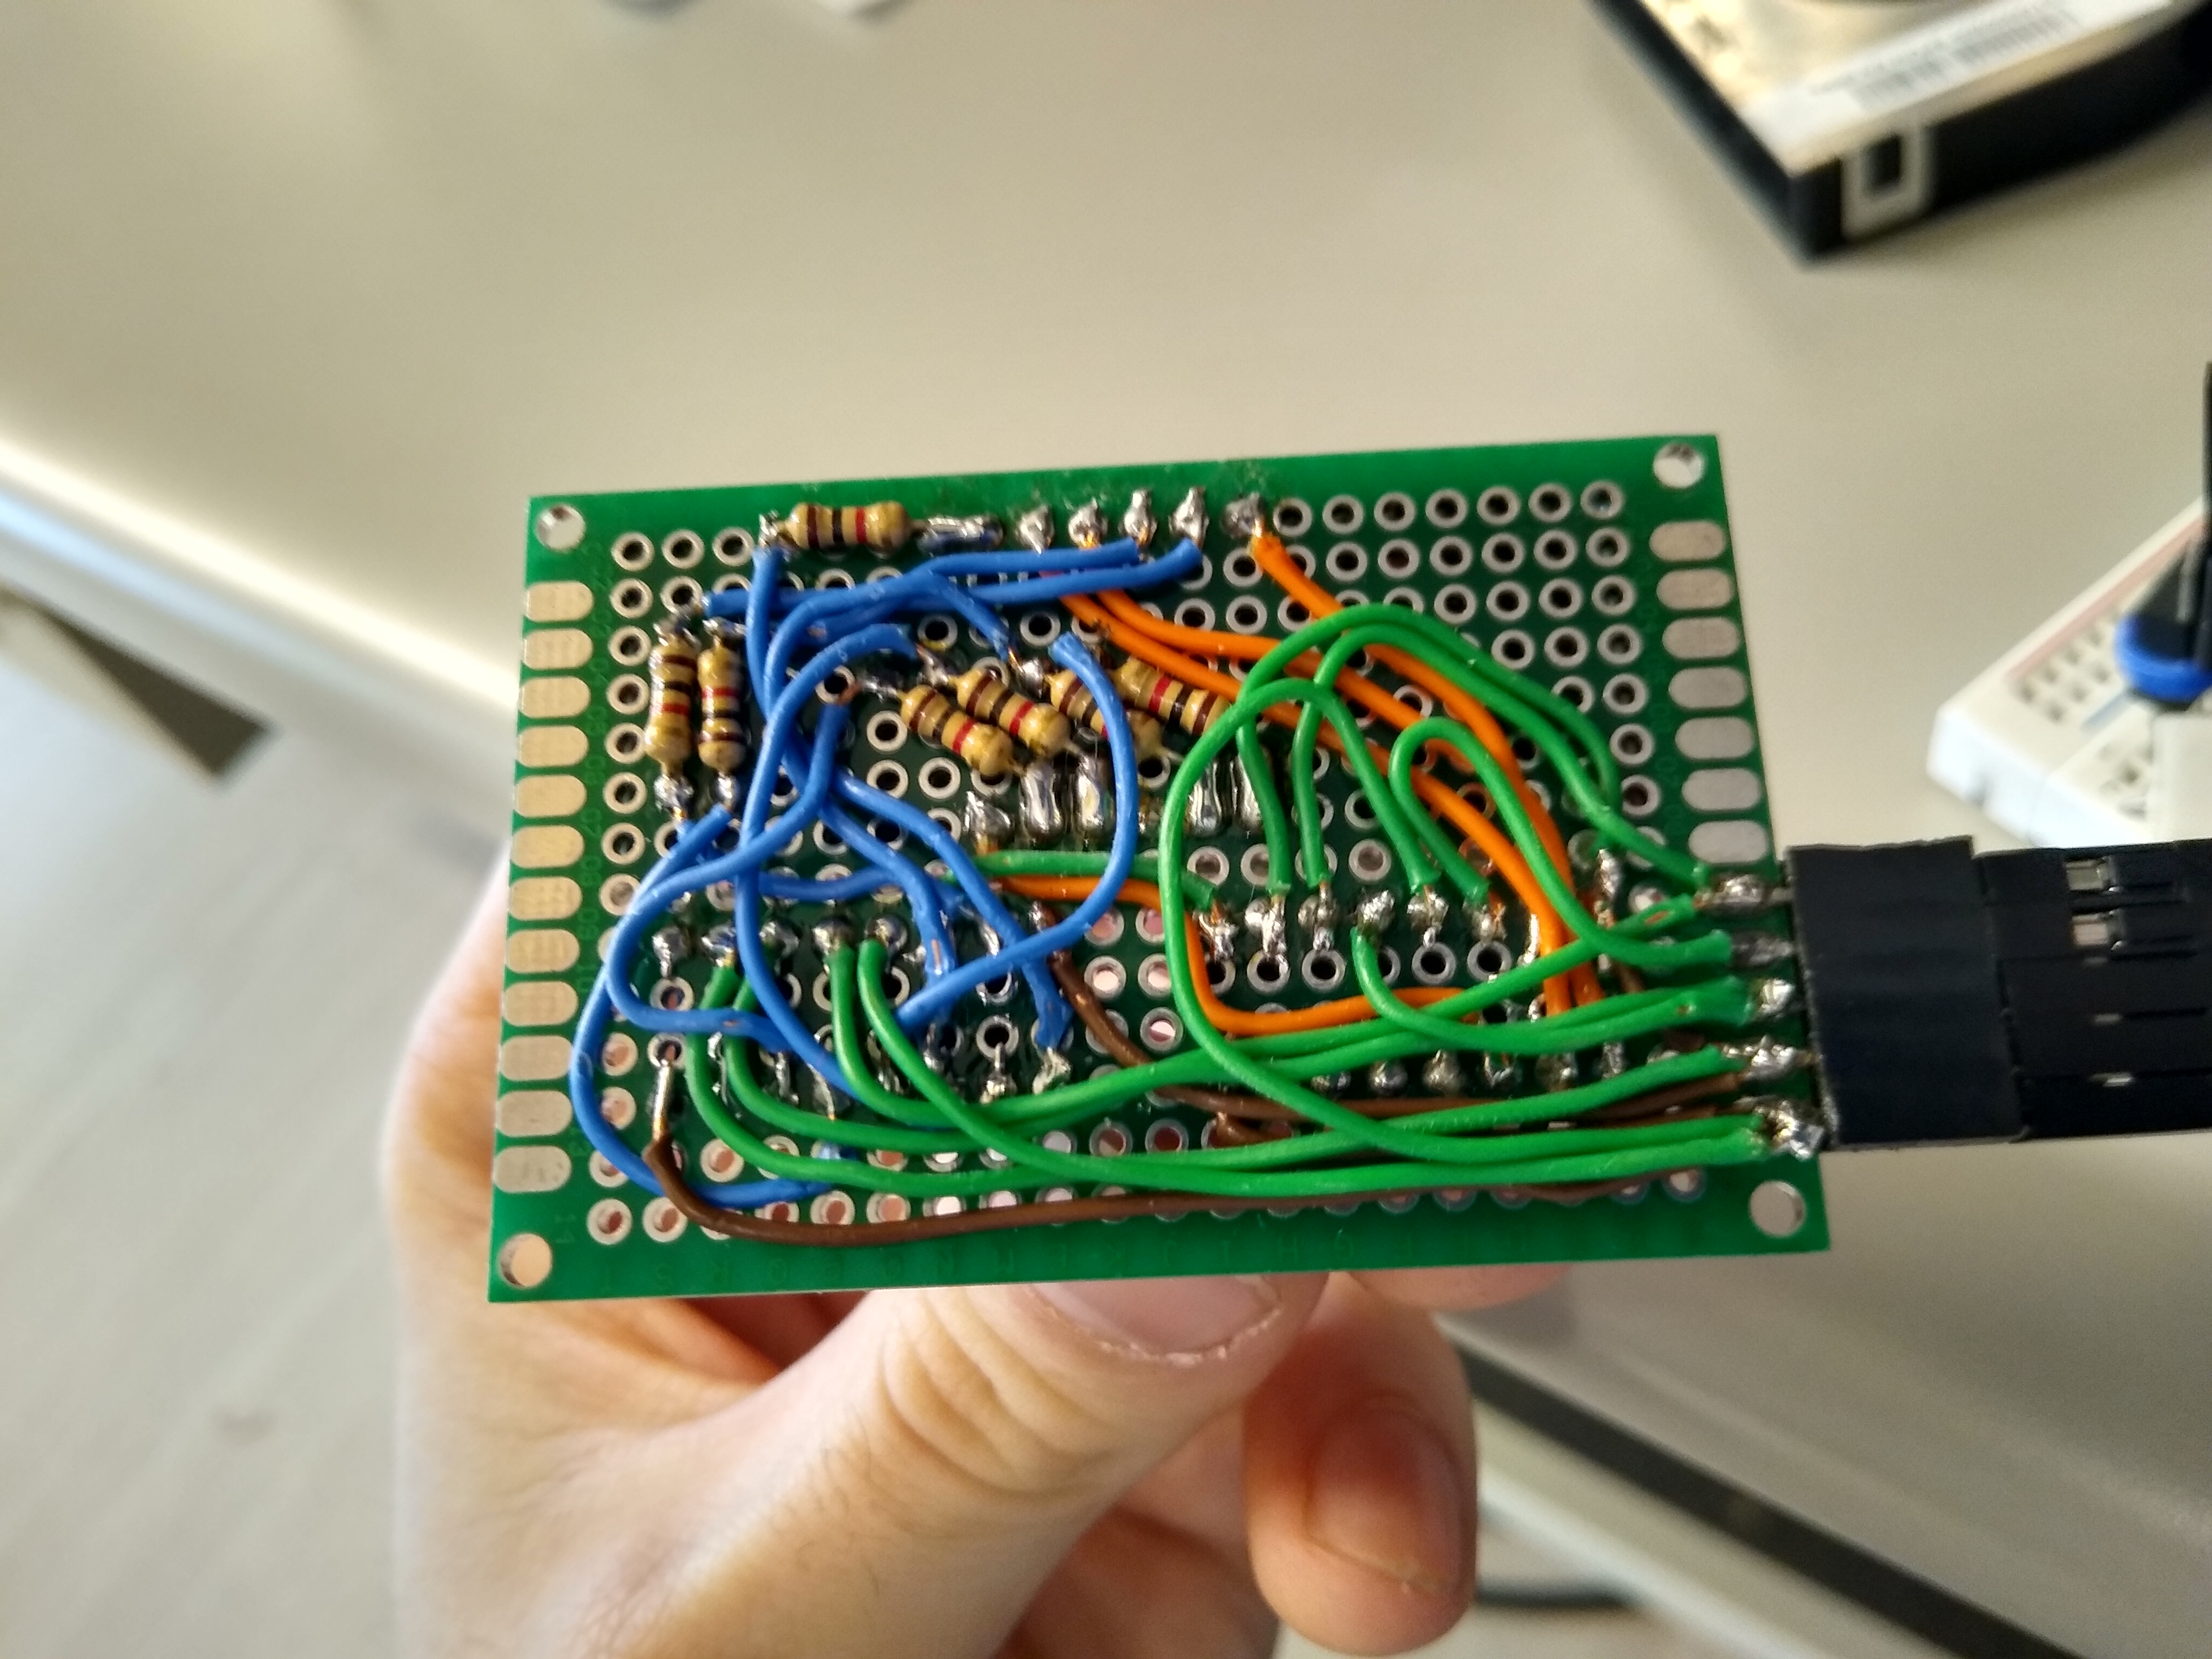
\includegraphics[width=0.9\textwidth]{boardphoto3.jpg}
\caption{7seg board back}
\label{fig:boardphoto2}
\end{figure}

\section{Key System Specifications}


This design operates off a single 5-12v supply. The fan, thermistor, and microcontroller all operate on 5v logic. A 5v linear voltage regulator was used off of the same 12v supply. 
\\
The specifications are as follows:\\
\begin{tabular}{|l||l|}
\hline	

Microcontroller            & Attiny13a \\ \hline
voltage                    & 3-12v       \\ \hline
File size					& 996 Bytes		\\ \hline
lowest usable temp			& 0 C			\\	\hline
Highest temp usable			& 63 C			\\	\hline
\end{tabular}
\\
Note that the temperature range is given so that it can fit on the 7seg display, and so that is easy to set using the potentiometer.

\section{System Description}

\subsection{Detailed Block Diagram}
Below is a more detailed image of the basic structure of the microcontroller and what it's interfacing with. 
\begin{figure}[H]
\centering
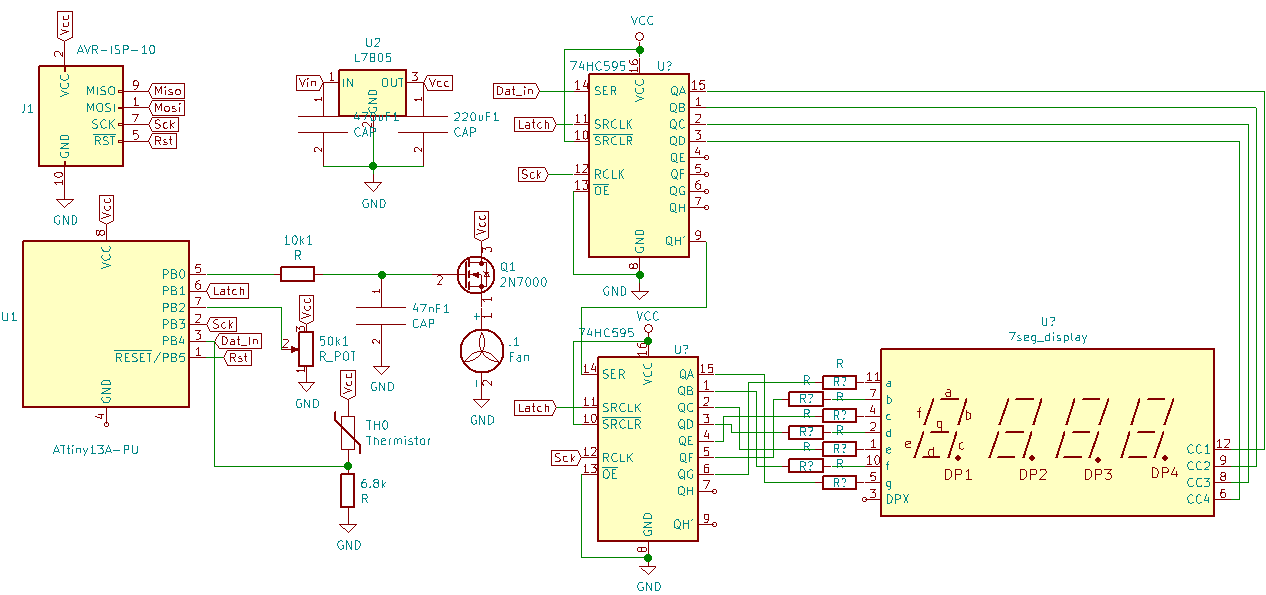
\includegraphics[width=\textwidth]{schem.png}
\caption{KiCad Schematic}
\label{fig:KiCadSchem}
\end{figure}
\subsection{Highlighted Devices}

\begin{itemize}
\item AtTiny13a-pu		-Microcontroller used for the fan controller.
\item NTCLE100E3		-Temperature-controlled resistor
\item 2N7000			-Fan driving transistor
\end{itemize}

\subsection{Attiny13a-pu}

This device is a low power 8-bit microcontroller offered by Atmel with 1 8-bit timer. In this project, an 8-bit timer was used in fast PWM mode to multiplex the display, used to read the thermistor, used to read the varistor, and used to time calculating the PID value at 5 Hz. 996 bytes of the 1 KB flash were used. 4 bytes of the 64 byte ram were used. The absolute maximum current consumption, sourcing or sinking, is 20 mA with a maximum of 200 mA for the entire package. 
\subsection{Thermistor}
This device is a through-hole two pin thermistor. This device has a temperature characteristic visible below:
\begin{equation}
\frac{1}{3.354016*10^{-3}+2.569850^{-4}*ln(R)}
\end{equation}
where R is resistance. This is the first two terms of the Steinhart and Hart Equation.
\\
Below the input voltage Vs. The temperature calculated is visible. Instead of making the microcontroller do several logarithms and float divisions, the equation was simplified to two equations. 
\begin{enumerate}
\item {T(v) = 21v - 17}
\item {T(v) = 45v - 106}
\end{enumerate}

\begin{figure}[H]
\centering
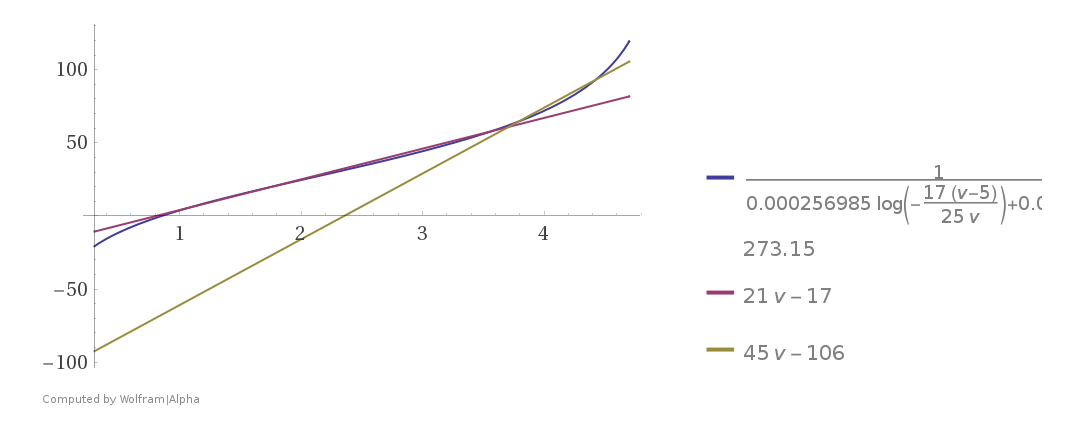
\includegraphics[width=0.9\textwidth]{characteristics.png}
\caption{Voltage vs temperature}
\label{fig:temp}
\end{figure}
\subsection{2N7000}
This device was used as a low side switch to switch the fan. The fan needed 100 mA, and that is well within the 250 mA max current rating. Any MOSFET with an $I_{max}$ higher than ~200 mA may be used.


\section{SYSTEM DESIGN THEORY}
This design required reading an analog voltage from the thermistor using an ADC, calculating the temperature, and set a PWM value for a fan. This occurs until power to the system is removed. The PWM value for the fan is set using a PID controller. The PID controller has a specific equation that is followed. This is visible below:
\begin{equation}
u = K_p e + K_i \int_0^t e dt + K_d \frac{d}{dt} e
\end{equation}
This is then modified so the microcontroller can easily compute it.\\
\begin{equation}
u = K_p e + K_i \Sigma_0^t  e + K_d( e - e[t-1])
\end{equation}
\\
This PID controller uses three calculations and sums the result. Initially, it calculates the error from a reference temperature. The error is then multiplied by a constant, and this is the Proportional component of the PID. For the integral, all of the past errors are summed up and multipled by a constant. For the D term, the previous error is subtracted from the current error, and multiplied by a third constant.
\\
Because of the limits of unsigned numbers, the p and i terms had to be kept positive. For example, if we just use the proportional term and if the current temperature is one bit over the reference temperature, an underflow will occur and the fan will be set to max speed.

\subsection{Design Requirement 1}

This design has one simple requirement: a fan needs to be set at a speed based off a read temperature. This was done successfully with this controller. There is some overshoot at lower temperatures (~25 deg) and it quickly reaches temperature. Near higher temperatures (~65 C), there is some oscillation because something as small as a slight draft can cause a 5 deg temperature change. These oscillations are typically within $\pm$ 1 degree C. 



%\section{Getting Started/How to use the device}
%\subsection{Connecting power}
%This is as easy as it sounds. Connect the following pins to Vcc and ground
%\begin{itemize}
%\item VCC		- Pin 7,21
%\item GND		- Pin 8,22
%\end{itemize} 
%Please note that the input voltage needs to be somewhere between 3v and 12v. The controller can operate below this, but the temperature reading will be skewed.
%\subsection{Connecting the thermistor}
%This is just as easy as connecting power. The thermistor needs to be connected to Vcc and ADC1 (pin 24). a 6800$\Omega$ resistor needs to be connected from ADC1 (pin 24) and ground. 
%\subsection{Connecting the fan}
%The fan is driven by a 2N7000 acting as a low side switch. Connect the fan to Vcc and the source of the MOSFET. Connect the gate to OC0A (pin 12), and the drain to ground.
%\section{Getting Started Software/Firmware}
%\subsection{Programming the device}
%Before this tutorial, you need to have avr-gcc, avrdude installed. \\
%First, you connect your favorite In-system-programmer in SPI. It should be 5v tolerant since that's what the circuit currently has.
%\begin{itemize}
%\item MISO		- Pin 6 (PB4)
%\item MOSI		- Pin 5 (PB3)
%\item RST		- Pin 1  (PC6)
%\item SCK		- Pin 7 (PB5)
%\item VCC		- Pin 8
%\item GND		- Pin 4
%\end{itemize}
%Following this, you need to make sure the device is connected. Open your favorite terminal and run  
%\begin{lstlisting}[language=bash]
%$ avrdude -c usbasp -p t13
%\end{lstlisting}
%The fuses should be E:FF, H:FF, L:7A. If not, refer to \href{http://heliosoph.mit-links.info/arduinoisp-reading-writing-fuses-attiny13a/}{here} for writing fuses.
%following this, in the "attiny13" folder, fun the following command:
%\begin{lstlisting}[language=bash]
%$ make program
%\end{lstlisting}
%This will program the device and verify the chip to make sure that it's programmed correctly. This program uses 996 bytes. The node should be completely setup and ready for use. If an issue is encountered and a solution cannot be found, please search \href{http://www.avrfreaks.net/}{AVRfreaks}. If an issue is still not found, feel free to make a post on that website, as it is one of the largest microcontroller communities on the planet.

%\section{Test Setup}
%For the test setup used in this appnote, nothing different was done from the previous section. 
%\subsection{Test Data}
%The PID controller was modeled in matlab, and it was found that the time constant for heating was 115 s. The time constant for cooling was 24s, and the time constant for both was 13s. This was plotted in matlab.

\section{Code Review}
\subsection{Initialization}
In the initalization, this code does quite a bit. First, it initializes timer 0 to fast PWM at 585 Hz with overflow interrupts enabled. Next, it sets the I/O register DDRB to 0xFB. This will change 585 times/second, which you will find out later. It then initializes almost all uint8\_ t s and uint16\_ t s to 0, and the loop starts. The ADC is initialized as it is used since the single shot mode does not seem to work with timer0 running. Every overflow, the display is updated one digit at a time. 
\subsection{Sensor Acquisition}
585 times per second, the microcontroller reads the thermistor. First, it initializes the ADC and reads the potentiometer, and goes to sleep. Upon waking up, it calculates the temperature by dividing by 4, and storing it. The microcontroller then reads the thermistor value. In this, it does something fancy. It uses the above 8-bit value and runs it through the following equation: $(uint8_t)(((uint16_t)105*ADCval)/256 - 17)$ This is just (0.4101*ADCval) - 17 but with division by a power of 2 and no floats to keep it more efficient. 
\subsubsection{Signal Conditioning}
Upon having both of these values as temperatures, it calculates the difference and sends that, along with the last data point to the PID function. This function is only executed every 117 timer 0 overflows, which comes out to 5 Hz. In this, the P was set to 50, which keeps the deadzone effect to a minimum, the I was set to 1, which is just enough to keep the error to a minimum with light oscillations, and the D term was 30, which acts as a boost to get the microcontroller out of a deadzome when changing between temperature values. The D term is not needed, but it seems to make a stronger response. 
\\
After calculating the PID value, the system sets the PWM appropriately. 
\subsection{Error Calculation}
The error was calculated by subtracting the current value from the goal value. Nothing was cone to condition this value.
\subsection{Control Calculation}

\begin{figure}[H]
\centering
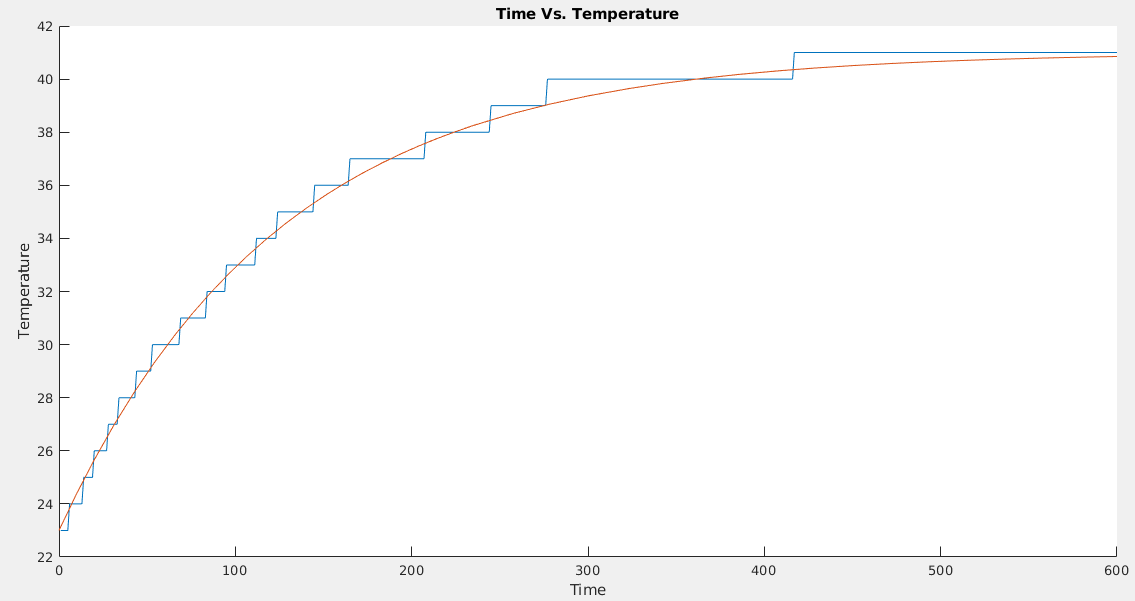
\includegraphics[width=0.9\textwidth]{Fan_off_R_t=0.png}
\caption{Regulator heating}
\label{fig:heat}
\end{figure}
In figure \ref{fig:heat} above, the regulator is heating and the fan is off. This is at 5v Vin. The time constant was found to be 115 seconds with a settling time of 462 seconds. 
\begin{figure}[H]
\centering
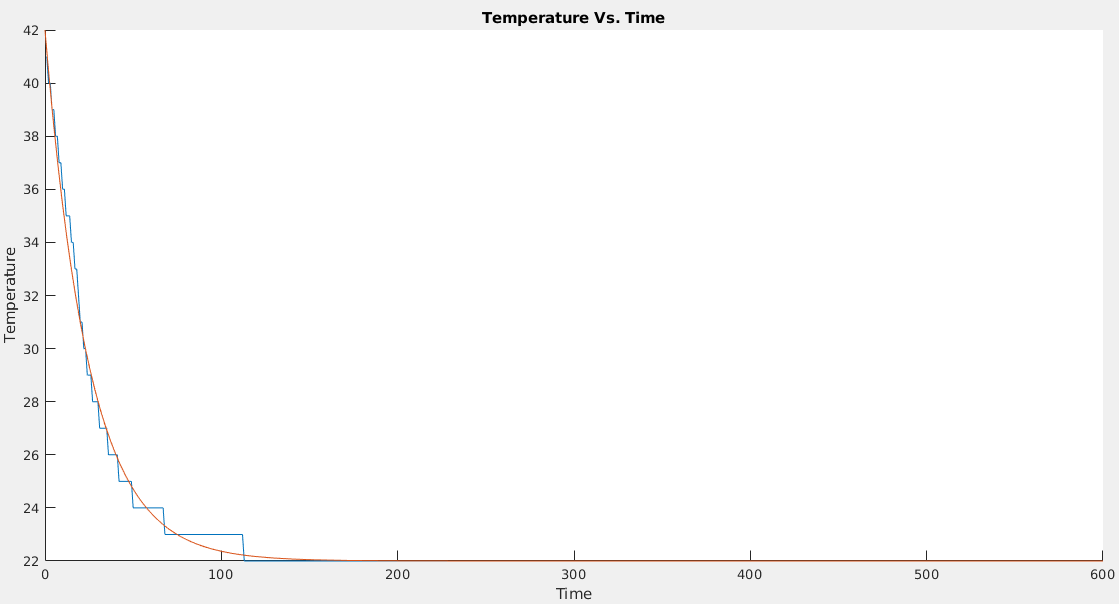
\includegraphics[width=0.9\textwidth]{Fan_t=0_Roff_t=0.png}
\caption{fan cooling}
\label{fig:cool}
\end{figure}
In figure \ref{fig:cool}, the regulator is turned off at t=0, fan cooling at t=0. The time constant was found to be 24 seconds, and the settling time was 116 seconds. 

\begin{figure}[H]
\centering
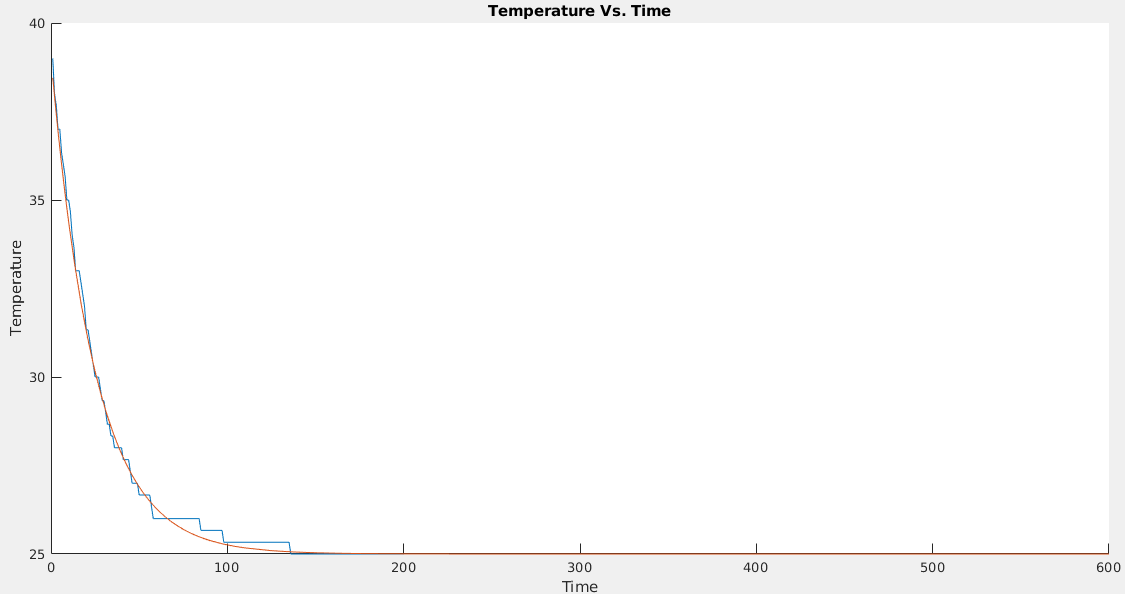
\includegraphics[width=0.9\textwidth]{Fan_t=0_R=on.png}
\caption{regulator heating and fan cooling}
\label{fig:heatcool}
\end{figure} 
In figure \ref{fig:heatcool}, the regulator is fully heated with a 5v input, and the fan is turned on at t=0. 
\\
\subsection{display}
In this system, the temperature is outputted over the 7seg display at 595.9 Hz per number, so 146.5 Hz overall for the 4 digits. This display had to be mapped out, with the first 8 bits controlling the anode and the 2nd 8 bits controlling the cathode. Fortunately, this was already done in the embedded final project that was done last semester. 
\\
\subsection{Matlab}
This system was attempted to be simulated in matlab. There were issues with the two different time constants for heating and cooling. This was attempted to be simulated in simulink, but almost any value would give a stable system with no oscillation, which was not the case in real life. This PID was tuned using the Ziegler-Nichols method, which involved first setting the I and D gains to zero, increasing the P gain until a sustained and stable oscillation (as close as possible) is obtained on the output. Then the critical gain Kc and the oscillation period Pc is recorded and the P, I, and D values adjusted accordingly. For P, I, and D, Kp becomes 0.65Kc, Ki becomes 0.5Pc, and Kd becomes 0.12Pd.
\subsection{filter}
No physical filter was implemented because it would potentially skew the values. The noise on any analog line is already low due to the relatively low resistance of the potentiometer (10k) and the relatively low resistance of the thermostor and accompanying resistor (6.8k). Since this system is completely linear, e.g. voltage fluctuations in the supply line will result in a proportional voltage fluctuations on an analog pin, any capacitor added would distort this linearity. If one was added, it would be an RC low-pass filter with a cutoff frequency of a few Hz to eliminate high frequency noise. 
\\
\\
A 2-sample moving average filter was implemented on this project. This filters both the potentiometer and the thermistor. Only 2 samples were used because if 4 were used, the project would become 1064 bytes, which is over the 1024-byte limit.


\subsection{Actuation}
The system actuates a small 5v fan that came from a 2006 HP laptop that was laying around. It has a deadzone that starts around 1.5 volts, which is great. This value is so low because the stator is much smaller than typical cooling fan designs. Since this is a small fan, it does not need to have too much torque, so this is the perfect application.

\section{Design Files}

\subsection{Schematics}

\begin{figure}[H]
\centering
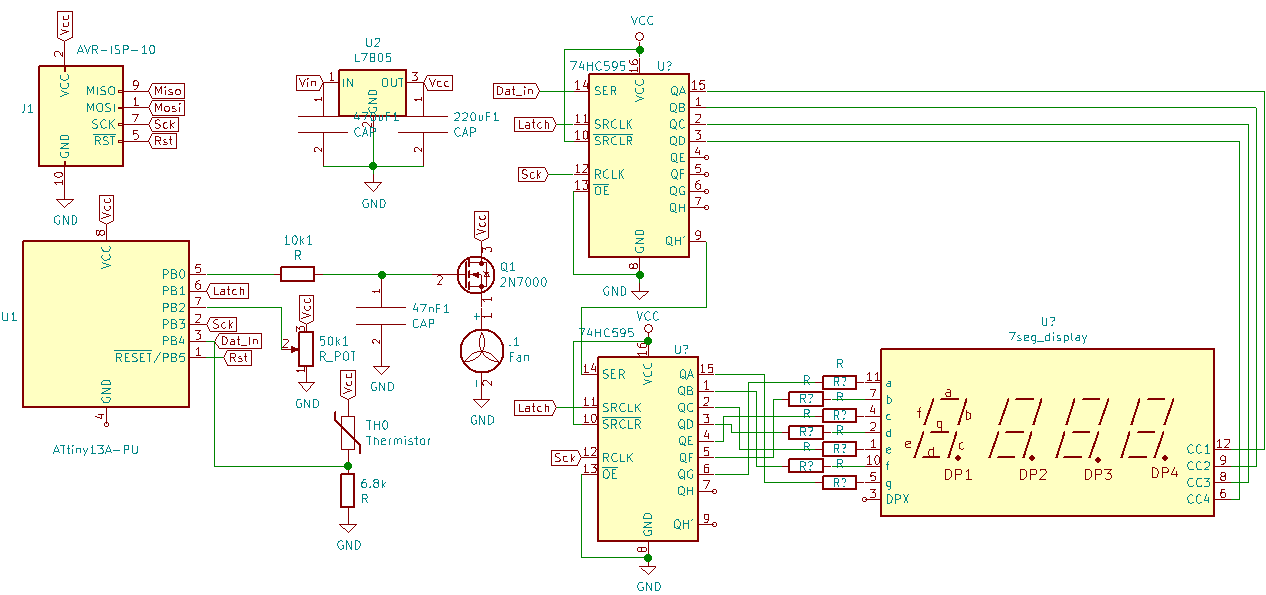
\includegraphics[width=0.9\textwidth]{schem.png}
\caption{Schematic of system}
\label{fig:schem}
\end{figure}
\subsection{Bill of Materials}
This bill of materials is priced in quantities of 1000. If surface mount components are used, price can be significantly reduced.\\
\begin{tabular}{|l|l|l|}
\hline	

 ITEM								&	QTY	&	PRICE/EA \\ \hline
 Attiny13a-pu						&	1	&	\$0.60 \\ \hline
 1/4 Carbon Film Res 6800$\Omega$ 	&	1	&	\$0.01 \\ \hline
 NTCLE100E3	 Thermistor				&	1	&	\$0.22	\\	\hline
 47 nF capacitor						&	1	&	\$0.02 \\ \hline
 220 uF capacitor					&	1	&	\$0.06	\\ \hline
 470 uF capacitor					&	1	&	\$0.08	\\ \hline
 35mm x 47mm breadboard				&	1	&	\$0.14 \\ \hline\hline
 TOTAL								&		&	\$1.13 \\ \hline

\end{tabular}

\subsection{Diptrace Project}
This project was made using KiCad. The schematic is visible in a github repository, which will be shared on request from Matt (Raineym5@studnets.rowan.edu). No board was produced in this project.
\subsection{Code}
The code below is the entire code, resulting in 996 bytes. Strangely, the comments would not post in LaTeX, so these were omitted.
\begin{verbatim}

#define F_CPU 8000000UL 
#include <avr/io.h>
#include <stdint.h>
#include <avr/interrupt.h>
uint8_t REF = 30,ovf_counter=0,ovf_flag=0,sregctr=0;
uint8_t receivedchars[] = {0,0,0,0};
const uint8_t 	kp 	= 50,
				ki 	= 1,
				kd 	= 30;
int16_t p=0,i=0,d=0;

void latch(void){
	PORTB |= (1<<PB1);
	asm("nop");
	PORTB &= ~(1<<PB1);
}
void Timer_Init(void){
	TCCR0A = (1<<COM0A1)|(1<<WGM01)|(1<<WGM00);
	TCCR0B = (1<<CS01)|(1<<CS00);
	OCR0A = 0;
	TIMSK0 = (1<<TOIE0);
}
void IO_init(void){
	DDRB = 0xFB;
}
uint8_t readADC_potentiometer(void){
	ADCSRA = (1<<ADEN)|(1<<ADPS2)|(1<<ADPS1)|(1<<ADIE);
	ADMUX = (1<<MUX0)|(1<<ADLAR);
	ADCSRA |= (1<<ADSC);
	asm("SEI");
	MCUCR = (1<<SE);
	asm("sleep");
	ADCSRA = 0;
	return ADCH;
}
uint8_t readADC_thermistor(void){

	ADCSRA = (1<<ADEN)|(1<<ADPS2)|(1<<ADPS1)|(1<<ADIE);
	PORTB &= ~(1<<PB4);
	DDRB &= ~(1<<PB4);
	ADMUX = (1<<MUX1)|(1<<ADLAR);
	ADCSRA |= (1<<ADSC);
		
	asm("SEI");
	MCUCR = (1<<SE);
	asm("sleep");

	DDRB |= (1<<PB4);
	ADCSRA = 0;
	return ADCH;
}
void send(uint8_t input){
	for(uint8_t i=0;i<8;i++){
		if((input & 0x01)== 0x01)
			PORTB |= (1<<PB4);
		else
			PORTB &= ~(1<<PB4);
		input = input>>1;
		PORTB |= (1<<PB3);
		PORTB &= ~(1<<PB3);
	}
}	


uint8_t PID_Error_PWM(int8_t error[2]){
	uint16_t total;
	
	p =  kp*error[0];//P term
	if(p >= 255)
		p = 255;
	if(p < 0)
		p=0;
		
	i = i + ki*error[0];
	if(i >= 200)
		i = 150;
	else if(i < 0)
		i=0;
		
	d =  kd * (error[1]-error[0]);
	if(p+i == 0)
		d=0;
	total = p+i+d;
	if(total >= 255)
		return 255;
	return (uint8_t)total;
}
uint8_t numtodisp(uint8_t disp){
	if(disp == 1)return 0x60;
	else if(disp == 2)return 0xDA;
	else if(disp == 3)return 0xF2;
	else if(disp == 4)return 0x66;
	else if(disp == 5)return 0xB6;
	else if(disp == 6)return 0xBE;
	else if(disp == 7)return 0xE0;
	else if(disp == 8)return 0xFE;
	else if(disp == 9)return 0xF6;
	return 0xFC;
}
void temp_to_disp(uint8_t temp,uint8_t bit){
	
	uint8_t counter = 0;
	while(temp >= 10){
		counter++;
		temp-=10;
	}		
	receivedchars[bit] = numtodisp(counter);
	receivedchars[bit+1] = numtodisp(temp);
	

}
uint8_t ADCtoTEMP(uint8_t ADCval){
		return (uint8_t)(((uint16_t)105*ADCval)/256 - 17);
}
ISR(TIM0_OVF_vect){
	if(ovf_counter >= 117){
		ovf_flag = 1;
		ovf_counter = 0;
	}else
		ovf_counter++;
	if(sregctr == 0x80){
		send( receivedchars[2]);
	}else if(sregctr == 0x40){
		send( receivedchars[3]);
	}else if(sregctr == 0x20){
		send( receivedchars[0]);
	}else if(sregctr == 0x10){
		send( receivedchars[1]);
	}else
		sregctr = 0x08;
	send(~sregctr);
	latch();
	if(sregctr == 0x80)
		sregctr = 0x08;

		sregctr = sregctr<<1;
}
ISR(ADC_vect){}
uint8_t PottoTemp(uint8_t pot){
	return pot>>2;
}
int main(void){

	DDRB = 0xFF;

	Timer_Init();

	IO_init();
	uint8_t realTemp[]={0,0},goalTemp_filtered = 0,realTemp_ADC = 0;
	uint8_t goalTemp_ADC = 0,goalTemp[] = {0,0},realTemp_filtered=0;
	int8_t error[] = {0,0};
	while(1){
		asm("SEI");
		MCUCR = (1<<SE);
		asm("sleep");
		
		goalTemp_ADC = readADC_potentiometer();
		realTemp_ADC = readADC_thermistor();
		goalTemp[0] = goalTemp[1];
		goalTemp[1] = PottoTemp(goalTemp_ADC);
		goalTemp_filtered = (goalTemp[0] + goalTemp[1])>>1; 
		
		realTemp[0] = realTemp[1];
		realTemp[1] = ADCtoTEMP(realTemp_ADC);
		realTemp_filtered = (realTemp[0] + realTemp[1])>>1; 
		temp_to_disp(goalTemp_filtered,0);
		temp_to_disp(realTemp_filtered,2);
		
		if(ovf_flag){
		ovf_flag=0;
		
		error[0] = realTemp_filtered - goalTemp_filtered;
		OCR0A = PID_Error_PWM(error);
		
		error[1] = error[0];
		}
	}
	return 0;
}
\end{verbatim}

\end{document}